\chapter{Machine Learning}

\section{Artificial Neural Networks}

\textit{Artificial Neural Networks} are mathematical models inspired by biological neural networks. They are composed of (layers of) connected neurons and characterized by processes changing their structure based on the flowing information during the \textit{learning} stage.

The first mention of this term is in McCulloch and Pitts' 1943 work \cite{McCulloch1943}, where they introduced a Threshold Logic Unit (or Linear Threshold Unit), able to implement simple boolean functions \ref{fig:TLU}.

\begin{figure}[H]
	\centering
	\begin{equation*}
		\begin{aligned}[c]
			TLU(\vec{x}) & = \phi \bigg( \sum_{i=1}^{n}{w_{i} \cdot x_{i}} \bigg) \\
			\phi(x)      & = x - \theta \geq 0
		\end{aligned}
		\quad
		\begin{aligned}[c]
			n      & = 2   \\
			\theta & = 1.5 \\
		\end{aligned}
		\quad
		\begin{aligned}[c]
			w_{1} & = 1.0 \\
			w_{2} & = 1.0
		\end{aligned}
	\end{equation*}
	\caption{Boolean logic AND implemented by a Threshold Logic Unit}
	\label{fig:TLU}
\end{figure}

\paragraph{Perceptron}

Rosenblatt introduced in 1958 the \textit{Perceptron}\cite{rosenblatt1958perceptron}, a linear binary classificator now considered the simplest feed-forward neural network.

It can be modeled as follows:

\begin{equation*}
	\begin{aligned}[c]
		f(\mathbf{x}) = \begin{cases}1 & \text{if }\ \mathbf{w} \cdot \mathbf{x} + b > 0,\\0 & \text{otherwise}\end{cases}
	\end{aligned}
\end{equation*}

\begin{equation*}
	\begin{aligned}[c]
		w = \begin{bmatrix}
			w_{1} & \cdots & w_{d} & b
		\end{bmatrix}
	\end{aligned}
	\quad
	\begin{aligned}[c]
		\vec{x} = \begin{bmatrix}
			x_{1}  \\
			\vdots \\
			x_{d}  \\
			1
		\end{bmatrix}
	\end{aligned}
\end{equation*}

\begin{figure}[H]
	\centering
	\begin{tikzpicture}
		\node[functions] (center) {};
		\node[below of=center,font=\scriptsize,text width=4em] {Activation function};
		\draw[thick] (0.5em,0.5em) -- (0,0.5em) -- (0,-0.5em) -- (-0.5em,-0.5em);
		\draw (0em,0.75em) -- (0em,-0.75em);
		\draw (0.75em,0em) -- (-0.75em,0em);
		\node[right of=center] (right) {};
		\path[draw,->] (center) -- (right);
		\node[functions,left=3em of center] (left) {$\sum$};
		\path[draw,->] (left) -- (center);
		\node[weights,left=3em of left] (2) {$w_2$} -- (2) node[input,left of=2] (l2) {$x_2$};
		\path[draw,->] (l2) -- (2);
		\path[draw,->] (2) -- (left);
		\node[below of=2] (dots) {$\vdots$} -- (dots) node[left of=dots] (ldots) {$\vdots$};
		\node[weights,below of=dots] (n) {$w_n$} -- (n) node[input,left of=n] (ln) {$x_n$};
		\path[draw,->] (ln) -- (n);
		\path[draw,->] (n) -- (left);
		\node[weights,above of=2] (1) {$w_1$} -- (1) node[input,left of=1] (l1) {$x_1$};
		\path[draw,->] (l1) -- (1);
		\path[draw,->] (1) -- (left);
		\node[weights,above of=1] (0) {$w_0$} -- (0) node[input,left of=0] (l0) {$1$};
		\path[draw,->] (l0) -- (0);
		\path[draw,->] (0) -- (left);
		\node[below of=ln,font=\scriptsize] {Inputs};
		\node[below of=n,font=\scriptsize] {Weights};
	\end{tikzpicture}
\end{figure}

\subsection{Activation Functions}
\begin{description}[leftmargin=!,labelwidth=\widthof{\bfseries The longest label}]
	\item[Logistic]
	      ${(1 + e^{-x})}^{-1}$
	\item[Hyperbolic]
	      $\tanh(x)$
	\item[Rectified Linear Unit (ReLU)]
	      $\max(0,\, x)$
	\item[Leaky ReLU]
	      $\max(0.01x,\, x)$
	\item[Parametric LReLU]
	      $\begin{cases}
			      \alpha x & \text{if } x \geq 0 \\
			      x        & \text{if } x < 0    \\
		      \end{cases}$
	\item[Exponential Linear Unit (ELU)]
	      $\begin{cases}
			      \alpha(e^x - 1) & \text{if } x \geq 0 \\
			      x               & \text{if } x < 0    \\
		      \end{cases}$
\end{description}

\begin{figure}
	\centerline{
		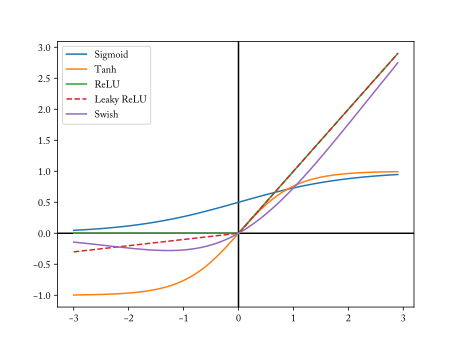
\includegraphics[width=0.4\paperwidth]{activation_fun_comparison}}
	\caption{Comparison of activation functions}
	\label{fig:activation_functions}
\end{figure}
